 \documentclass[10pt, letterpaper]{article}
\usepackage[top=80pt,bottom=80pt,left=60pt,right=60pt]{geometry}
\usepackage{tabularx}
\usepackage{float}
\usepackage{amsmath} % for boxing equations
\usepackage{titling}
\newcommand{\subtitle}[1]{
  \posttitle{
    \par\end{center}
    \begin{center}\large#1\end{center}
    \vskip0.5em}
}
\usepackage{tikz}
\usepackage[section]{placeins}
\usepackage[utf8]{inputenc}
\usepackage{pgfplots} % for table
\usepackage{pgfplotstable} % for linear regression
\usepackage{csvsimple}
\usepackage{subfig}

\begin{document}

  \title{Internal Assessment: The Impact of the Sphere's Radius on the Sphere's Angular Velocity}
  \subtitle {IB Physics II Period 6, Dr. Petach}
  \date{19 October 2015}
  \author{Jackson Chen}
  \maketitle

  \section{Exploration}

    \subsection{Research}

    The aim of the experiment is to investigate the relationship between radius and
    angular velocity for the linear motion of a sphere unraveling from a string at a
    fixed height. This will be done by changing the radius of the sphere that is being
    dropped through the use of various sizes balls. They are then unraveled from the string
    and fall through a photogate, which measures their linear velocity.
    The purpose of the string is to cause the ball to rotate while falling, due to the
    nature of its unraveling motion.

    Prior to the experiment, I derived a relationship between the radius and the angular
    velocity of the rotational motion of the falling ball by using the law of conservation of
    energy. Section \ref{sssec:derivation} will more specifically detail the derivation.
    The derived relationship predicted that radius and angular velocity will follow an inverse relationship.
    The experiment itself was to test whether Newtonian physics upheld this inverse
    relationship with tangible experimentation.

    \subsection{Personal Engagement}

    I have always been a fan of yo-yo's. One day while playing with a yo-yo, I noticed how
    quickly the yo-yo was spinning, which was made especially conspicuous by the bright design
    on the side of the yo-yo. I became curious, did the size of the yo-yo affect how quickly
    it spun? I took a smaller yo-yo and noticed that it seemed to spin more quickly.
    However, this was just a casual observation, not performed under standard experimentation
    conditions. Interested in seeing if this was truly the case, I came up with my research
    question: does the radius of a sphere affect its angular velocity?

    \subsection{Variables}
    The independent variable is the radius of the sphere. The dependent variable is the
    angular velocity of the ball as it passes through the photogate. The controlled variables
    include the height of the initial position of the ball that is attached to the clamp,
    material of the string, the photogate, and the properties of the surrounding environment.

    \subsection{Apparatus}
    \begin{itemize}
      \item Photogate
      \item Four different sized balls that are relatively uniform spheres
      \item String
      \item DataWorks software that reads data from the photogate
      \item Ring stand with clamp
      \item Meter stick
    \end{itemize}

    \subsection{Procedure}
    \begin{enumerate}
      \item Attach a clamp to a ringstand
      \item Place a photogate toward the bottom of the ringstand so that the ball will drop through it.
      \item Connect the photogate to the DataWorks software, such that it reads the linear velocity of the falling ball
      \item Measure the height difference between the placement of the clamp and the photogate along the ring stand using a meter stick
      \item Pick a ball, measure its radius using a meter stick
      \item Tie one end of the string to a clamp attached to a ring stand, and the other end around the ball
      \item Carefully wrap the string around the ball until the ball is level with the clamp
      \item Drop the ball so that it falls through the photogate
      \item Record the linear velocity that is measured by the photogate
      \item Repeat steps 6 to 9 for six trials
      \item Repeat steps 5 through 10 for the four different balls
    \end{enumerate}

    \subsection{Experiment Setup}
    \begin{figure}[!htb]
      \centering
      \parbox{2.75in} {
        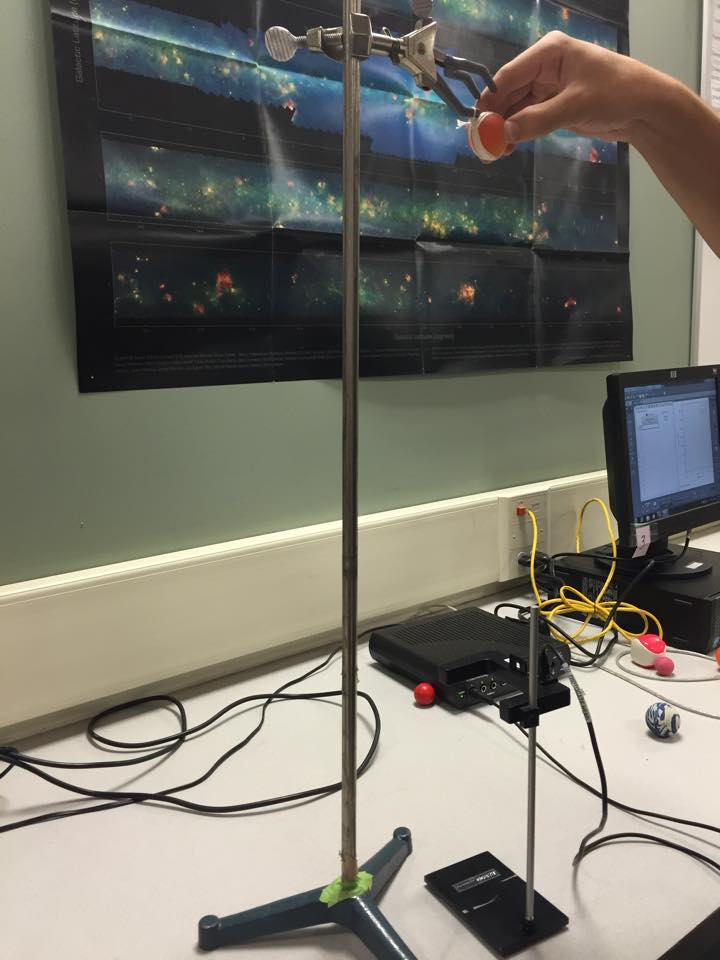
\includegraphics[scale=0.233]{img/setup.jpg}
        \caption{Picture of the experiment setup}
      }
      \begin{minipage}{2.75in}
        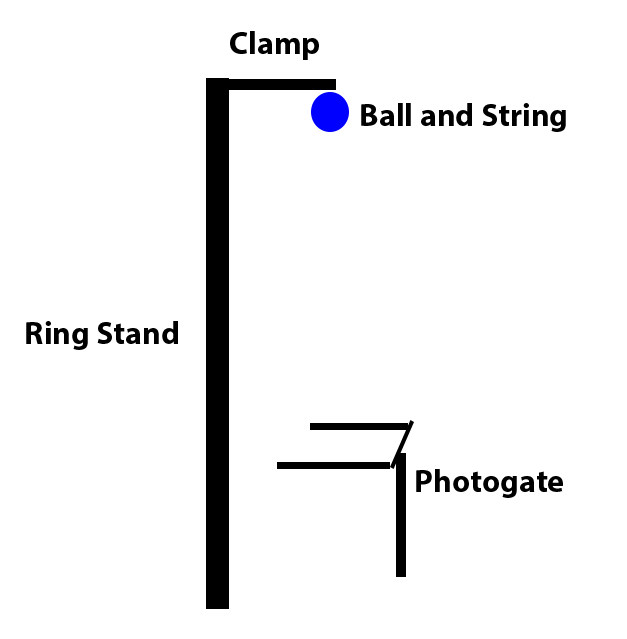
\includegraphics[scale=0.7]{img/apparatus.png}
        \caption{Diagram of the experiment setup}
      \end{minipage}
    \end{figure}

    \subsection{Data Collection}
      \begin{table}[H]
      \centering
      \begin{tabularx}{\linewidth}{>{\centering\arraybackslash}X>{\centering\arraybackslash}X>{\centering\arraybackslash}X }
        \hline \textbf{Trial} & \textbf{Radius (cm)} & \textbf{Linear Velocity (m/s)} \\ \hline
                1             & $2.34 \pm 0.05$      &  1.86 \\ \hline
                2             & $2.34 \pm 0.05$      &  1.81 \\ \hline
                3             & $2.34 \pm 0.05$      &  3.10 \\ \hline
                4             & $2.34 \pm 0.05$      &  2.50 \\ \hline
                5             & $2.34 \pm 0.05$      &  2.87 \\ \hline
                6             & $2.34 \pm 0.05$      &  2.20 \\ \hline
      \end{tabularx}
      \caption{Data for six trials with ball radius of 2.34 cm and height of $50.00 \pm 0.05$ cm.}
      \end{table}

      \begin{table}[H]
      \centering
      \begin{tabularx}{\linewidth}{>{\centering\arraybackslash}X>{\centering\arraybackslash}X>{\centering\arraybackslash}X }
        \hline \textbf{Trial} & \textbf{Radius (cm)} & \textbf{Linear Velocity (m/s)} \\ \hline
                1             &	$1.90 \pm 0.05$      & 2.12 \\ \hline
                2             &	$1.90 \pm 0.05$      & 2.38 \\ \hline
                3             &	$1.90 \pm 0.05$      & 2.98 \\ \hline
                4             &	$1.90 \pm 0.05$      & 2.23 \\ \hline
                5             &	$1.90 \pm 0.05$      & 2.35 \\ \hline
                6             &	$1.90 \pm 0.05$      & 2.23 \\ \hline
      \end{tabularx}
      \caption{Data for six trials with ball radius of 1.90 cm and height of $50.00 \pm 0.05$ cm.}
      \end{table}

      \begin{table}[H]
      \centering
      \begin{tabularx}{\linewidth}{>{\centering\arraybackslash}X>{\centering\arraybackslash}X>{\centering\arraybackslash}X }
        \hline \textbf{Trial} & \textbf{Radius (cm)} & \textbf{Linear Velocity (m/s)} \\ \hline
                1             &	$1.69 \pm 0.05$      &	3.32 \\ \hline
                2             &	$1.69 \pm 0.05$      &	3.18 \\ \hline
                3             &	$1.69 \pm 0.05$      &	2.22 \\ \hline
                4             &	$1.69 \pm 0.05$      &	3.91 \\ \hline
                5             &	$1.69 \pm 0.05$      &	2.85 \\ \hline
                6             &	$1.69 \pm 0.05$      &	3.63 \\ \hline
      \end{tabularx}
      \caption{Data for six trials with ball radius of 1.69 cm and height of $50.00 \pm 0.05$ cm.}
      \end{table}

      \begin{table}[H]
      \centering
      \begin{tabularx}{\linewidth}{>{\centering\arraybackslash}X>{\centering\arraybackslash}X>{\centering\arraybackslash}X }
        \hline \textbf{Trial} & \textbf{Radius (cm)} & \textbf{Linear Velocity (m/s)} \\ \hline
               1              &	$1.40 \pm 0.05$      &	2.91 \\ \hline
               2              &	$1.40 \pm 0.05$      &	3.62 \\ \hline
               3              &	$1.40 \pm 0.05$      &	3.62 \\ \hline
               4              &	$1.40 \pm 0.05$      &	2.31 \\ \hline
               5              &	$1.40 \pm 0.05$      &	3.67 \\ \hline
               6              &	$1.40 \pm 0.05$      &	3.41 \\ \hline
      \end{tabularx}
      \caption{Data for six trials with ball radius of 1.40 cm and height of $50.00 \pm 0.05$ cm.}
      \end{table}
  \section{Analysis}

    \subsection{Deriving the relationship between radius and angular velocity} \label{sssec:derivation}

      A relationship can be found between radius and angular velocity by using the law of conservation of energy.
      Effects of thermal energy (friction) from the string are negligible.
      \[ GPE = KE_{T} + KE_{R}\]
      \[ mgh = \frac{1}{2}mv^2 + \frac{1}{2}I \omega ^2 \]
      \[ mgh = \frac{1}{2}m(R \omega )^2 + \frac{1}{2} \left( \frac{2}{5}mR^2 \right) \omega ^2 \]
      \[ mgh = \frac{1}{2}mR^{2} \omega ^2 + \frac{1}{5}mR^{2} \omega ^2 \]
      The masses can be eliminated:
      \[ gh = \frac{7}{10}R^2 \omega ^2 \]
      \[ \omega ^2 = \frac{10gh}{7R^2} \]
      \[ \omega = \sqrt{\frac{10gh}{7R^2}} \]
      \begin{equation}
        \boxed{ \omega = \frac{1}{R} \cdot \sqrt{\frac{10gh}{7}} }
      \end{equation}

    \subsection{Averaging the six trials for each ball size and finding uncertainty}
      Uncertainty for linear velocity can be calculated by dividing the linear velocity range by 2.
      Calculations for the average linear velocity and uncertainty for the four ball sizes will
      be shown below: \\

      For ball with radius 2.34 cm:
      \[ \frac{3.10 - 1.81}{2} = \pm 0.65  \]
      \[ v = \frac{1.86 + 1.81 + 3.10 + 2.50 + 2.87 + 2.20}{6} = 2.39 \pm 0.65 \frac{m}{s} \]

      For ball with radius 1.90 cm:
      \[ \frac{2.98 - 2.12}{2} = \pm 0.43  \]
      \[ v = \frac{2.12 + 2.38 + 2.98 + 2.23 + 2.35 + 2.23}{6} = 2.38 \pm 0.43 \frac{m}{s} \]

      For ball with radius 1.69 cm:
      \[ \frac{3.91 - 2.22}{2} = \pm 0.85  \]
      \[ v = \frac{3.32 + 3.18 + 2.22 + 3.91 + 2.85 + 3.63}{6} = 3.19 \pm 0.85 \frac{m}{s} \]

      For ball with radius 1.40 cm:
      \[ \frac{3.67 - 2.31}{2} = \pm 0.68  \]
      \[ v = \frac{2.91 + 3.62 + 3.62 + 2.31 + 3.67 + 3.41}{6} = 3.26 \pm 0.68 \frac{m}{s} \]


    \subsection{Calculating angular velocity}
      Using the data from the experiment, the calculated angular velocity can be found from
      the linear velocity that is measured by the photogate, as shown in Equation 2.
      \begin{equation}
        \omega _{calc} = \frac{v}{r}
      \end{equation}
      The theoretical angular velocity can be found using Equation 1. Calculations for these
      two $\omega $ values will be shown below: \\

      For ball with radius 2.34 cm:
      \[ \omega _{theoret} = \frac{1}{0.0234} \cdot \sqrt{\frac{10*9.8*0.5000}{7}} = 113.1 \frac{rad}{s} \]
      \[ \omega _{calc} = \frac{2.39 \pm 0.65}{0.0234} = 100 \pm 30 \frac{rad}{s} \]

      For ball with radius 1.90 cm:
      \[ \omega _{theoret} = \frac{1}{0.0190} \cdot \sqrt{\frac{10*9.8*0.5000}{7}} = 139.3 \frac{rad}{s} \]
      \[ \omega _{calc} = \frac{2.38 \pm 0.43}{0.0190} = 130 \pm 20 \frac{rad}{s} \]

      For ball with radius 1.69 cm:
      \[ \omega _{theoret} = \frac{1}{0.0169} \cdot \sqrt{\frac{10*9.8*0.5000}{7}} = 156.6 \frac{rad}{s} \]
      \[ \omega _{calc} = \frac{3.19 \pm 0.85}{0.0169} = 190 \pm 50 \frac{rad}{s} \]

      For ball with radius 1.40 cm:
      \[ \omega _{theoret} = \frac{1}{0.0140} \cdot \sqrt{\frac{10*9.8*0.5000}{7}} = 189.0 \frac{rad}{s} \]
      \[ \omega _{calc} = \frac{3.26 \pm 0.68}{0.0140} = 230 \pm 50 \frac{rad}{s} \]


      \begin{table}[H]
      \centering
      \begin{tabularx}{\linewidth}{>{\centering\arraybackslash}X>{\centering\arraybackslash}X>{\centering\arraybackslash}X>{\centering\arraybackslash}X>{\centering\arraybackslash}X }
        \hline \textbf{Radius (m)} & \textbf{$v$ (m/s)} & \textbf{ $\omega _{calc}$ (rad/s)} & \textbf{ $\omega _{theoret}$ (rad/s)} \\ \hline
                $0.0234 \pm 0.0005$     &	 $2.39 \pm 0.65$        & $ 100 \pm 30$          & 113.1  \\ \hline
                $0.0190 \pm 0.0005$     &	 $2.38 \pm 0.43$        & $ 130 \pm 20$          & 139.3  \\ \hline
                $0.0169 \pm 0.0005$     &	 $3.19 \pm 0.85$        & $ 190 \pm 50$          & 156.6  \\ \hline
                $0.0140 \pm 0.0005$     &	 $3.26 \pm 0.68$        & $ 230 \pm 50$          & 189.0  \\ \hline
      \end{tabularx}
      \caption{Combined table with the average linear velocities, calculated and theoretical angular velocities}
      \label{tab:agg}
      \end{table}

    \subsection{Analyzing experiment evidence for angular velocity versus radius}

      \begin{figure}[H]
        \centering
        \begin{tikzpicture}
          \begin{axis}[
            legend pos=outer north east,
            title={Calculated Angular Velocity vs Radius for a Ball Dropped From a String},
            xlabel={Radius (m)},
            ylabel={Calculated Angular Velocity (rad/s)},
            xmin = 0.01,
            xmax = 0.03,
            ymax = 300,
            ymin = 50,
            scale = 1.3
            ]

            \addplot[scatter, only marks,
                  error bars/.cd,
                      y dir=both,
                      y explicit,
                      x dir=both,
                      x explicit,
              ] table[x=X,y=Y,y error=Y_error, x error = X_error] {data/combined.dat};
            \addplot [thick, red] table[
                y={create col/linear regression={y=Y}}
            ] % compute a linear regression from the input table
            {data/combined.dat};
            \addplot [blue, no markers] coordinates {(0.0145,280) (0.0229,70)};
            \addplot [green, no markers] coordinates {(0.0135,180) (0.0239,130)};

            \addlegendentry{Data}
            \addlegendentry{%
            $ y = \pgfmathprintnumber{\pgfplotstableregressiona} \cdot x
                    \pgfmathprintnumber[print sign]{\pgfplotstableregressionb}$}}
            \addlegendentry{$y = - 25000 \cdot x + 624.5$}
            \addlegendentry{$y = - 4807 \cdot x+ 244.9$}
          \end{axis}
        \end{tikzpicture}
        \caption{Graph of $\omega _{calc}$ vs radius with line of best fit, maximum slope, and minimum sloped lines.}
        \label{fig:calc}
      \end{figure}

      \begin{figure}[H]
        \centering
        \begin{tikzpicture}
          \begin{axis}[
            legend pos=outer north east,
            title={Theoretical Angular Velocity vs Radius for a Ball Dropped From a String},
            xlabel={Radius (m)},
            ylabel={Theoretical Angular Velocity (rad/s)},
            xmin = 0.01,
            xmax = 0.03,
            ymax = 200,
            ymin = 100,
            scale = 1.3
            ]

            \addplot[scatter, only marks,
                  error bars/.cd,
                      y dir=both,
                      y explicit,
                      x dir=both,
                      x explicit,
              ] table[x=X,y=Y,y error=Y_error, x error = X_error] {data/theoret.dat};
            \addplot [thick, red] table[
                y={create col/linear regression={y=Y}}
            ] % compute a linear regression from the input table
            {data/theoret.dat};

            \addlegendentry{Data}
            \addlegendentry{%
            $ y = \pgfmathprintnumber{\pgfplotstableregressiona} \cdot x
                    \pgfmathprintnumber[print sign]{\pgfplotstableregressionb}$}}
          \end{axis}
        \end{tikzpicture}
        \caption{Graph of $\omega _{theoret}$ vs radius with line of best fit.}
        \label{fig:theoret}
      \end{figure}

      From Figure \ref{fig:calc}, the steepest, or maximum, slope is -25000 and the minimum -4807.
      The best fit line slope is -14277. \\\\
      The uncertainty above the best fit line is $25000 - 14277 = 10723$. The negative can be disregarded
      because it is unnecessary when calculating uncertainty. \\
      The uncertainty below the best fit line is $4807 - 14277  = -9470$ \\\\
      The slope of the set of data points, including uncertainty is
      $-14277 \cdot \frac{10723}{-9470} = \boxed{ -14000 \pm 1000}$

  \section{Evaluation}
    \subsection{Percent Error Analysis}
    The slope means that an increasing radius decreases the angular velocity by a proportionality factor
    of $14000 \frac{m \cdot s}{rad}$ with an uncertainty of $\pm 1000$. \\

    According to the slope of the best fit line in Figure \ref{fig:theoret},
    which is based on $\omega _{theoret}$ values from Table \ref{tab:agg},
    the true proportionality factor should be 8000. Therefore a percent error analysis
    can be performed on the slope:
    \[ \frac{|8000 - 14000 \pm 1000|}{8000} \cdot 100 = 80 \pm 10 \% \]

    \subsection{Conclusion} \label{sec:conclusion}

    The relationship between radius and angular velocity is supported by the data, since the theoretical
    value for the slope of angular velocity versus radius is between the minimum and maximum
    values of the experiment. However, the errors involved were rather significant due to the large
    percent error, 80\% .

    A potential source is error is the shape of the balls that were used in the experiment. Some
    of the balls used were not completely spherical in shape, and had noticeable edges on the
    surface. This would have impacted the angular velocity, because the inertia used in the
    calculation was based on a spherical object. Secondly, the string that the ball unraveled
    from was uneven in width throughout its length due to the uneven distribution of mass. Some parts of the
    string also began to be worn out as the experiment continued. This would have affected the ball's path
    as it unraveled by changing the ball's trajectory and ultimately the height it fell.
    Finally, another source of error may stem from the software and photogate not measuring the
    angular velocity at fine enough time intervals. The graphs generated by the software displayed a
    spike when the ball passed through the photogate's sensors, but the point was very discrete. The lack
    of continuity makes it difficult to tell where precisely the spike was measured, and if it was
    measured in the most accurate location possible.

    \subsection{Improvements}

    There are many improvements that could be made to this experiment to fix many of the sources of error
    identified in Section \ref{sec:conclusion}. Firstly, balls that are visibly uniform should be picked
    for future experiments. This would mitigate the irregularity in ball shape, which would effect the angular
    velocity. In addition, a thinner string made out of a different material could be used to minimize
    uneven widths of the string at different points along its length. Furthermore, this experiment
    ignored the effects of thermal energy when deriving a relationship between radius and angular velocity,
    but future experimentation could take frictional force into consideration to provide even
    more accurate results. Finally, a different photogate could have been used to read data at
    much shorter intervals, and to ultimately allow for a more continuous time versus velocity graph.

\end{document}
